% Compile from the repository root with tectonic reports/final_project_report.tex
\documentclass[11pt,a4paper]{article}
\usepackage[a4paper,top=24mm,bottom=23mm,left=24mm,right=24mm,headheight=14pt,headsep=9mm,footskip=12mm]{geometry}
\usepackage{lmodern}
\usepackage{fontspec}
\setmainfont{texgyrepagella}[
  Extension=.otf, UprightFont=*-regular, ItalicFont=*-italic,
  BoldFont=*-bold, BoldItalicFont=*-bolditalic
]
\setsansfont{texgyreheros}[
  Extension=.otf, UprightFont=*-regular, ItalicFont=*-italic,
  BoldFont=*-bold, BoldItalicFont=*-bolditalic
]
\usepackage[protrusion=true,expansion=false]{microtype}
\usepackage[table]{xcolor}
\usepackage{booktabs,tabularx}
\usepackage{fancyhdr,titlesec}
\usepackage{etoolbox}
\usepackage{tikz}
\usetikzlibrary{positioning}
\usepackage{hyperref}

\definecolor{Ink}{HTML}{202B39}
\definecolor{Navy}{HTML}{163B63}
\definecolor{Blue}{HTML}{245D8E}
\definecolor{Muted}{HTML}{425974}
\definecolor{Rule}{HTML}{BBCCDD}
\definecolor{Wash}{HTML}{E8F0FA}
\definecolor{PaperTint}{HTML}{F2F6FB}

\hypersetup{
  pdftitle={Does Grounding Decay with Distance?},
  pdfauthor={Varun Patil, Harshal Bhansali, Deepti Koranga},
  pdfsubject={Causal explanations of Indian macroeconomic news},
  colorlinks=true, urlcolor=Blue, linkcolor=Blue, citecolor=Blue,
  bookmarksnumbered=true
}

\setlength{\parindent}{0pt}
\setlength{\parskip}{9pt plus 1pt}
\setlength{\emergencystretch}{1em}
\widowpenalty=10000
\clubpenalty=10000
\raggedbottom

\newcommand{\runninglabel}{}
\newcommand{\reportpage}[1]{\newpage\renewcommand{\runninglabel}{#1}}
\newcommand{\smalllabel}[1]{{\sffamily\bfseries\fontsize{8.5}{11}\selectfont\addfontfeatures{LetterSpace=6}\MakeUppercase{#1}}}
\pagestyle{fancy}
\fancyhf{}
\fancyhead[L]{\fontsize{9.4}{12}\selectfont\itshape\color{Navy}Does Grounding Decay with Distance?}
\fancyhead[R]{\fontsize{9.4}{12}\selectfont\color{Muted}\runninglabel}
\fancyfoot[C]{\fontsize{10}{13}\selectfont\color{Navy}\thepage}
\renewcommand{\headrule}{%
  {\color{Rule}\hrule height 0.45pt width\headwidth}\vskip-0.45pt\relax}
\fancypagestyle{opening}{\fancyhead{}\renewcommand{\headrule}{}}

\titleformat{\section}
  {\color{Navy}\rmfamily\bfseries\fontsize{18}{23}\selectfont}
  {\textcolor{Blue}{\thesection}}{0.7em}{}
\titleformat{\subsection}
  {\color{Navy}\rmfamily\bfseries\fontsize{12}{16}\selectfont}
  {\textcolor{Blue}{\thesubsection}}{0.7em}{}
\titlespacing*{\section}{0pt}{19pt}{11pt}
\titlespacing*{\subsection}{0pt}{18pt}{3pt}

\newcolumntype{L}[1]{>{\hsize=#1\hsize\linewidth=\hsize\raggedright\arraybackslash}X}
\newcommand{\tablehead}[1]{\textbf{#1}}
\newcounter{reporttable}
\newenvironment{reporttable}[1]{%
  \par\addvspace{14pt}\noindent\begin{minipage}{\linewidth}
  \refstepcounter{reporttable}%
  {\rmfamily\fontsize{10.5}{13.5}\selectfont
    \textcolor{Navy}{\bfseries Table \thereporttable.}\enspace #1}\par\vspace{8pt}%
  \rmfamily\fontsize{10.2}{13.5}\selectfont
  \renewcommand{\arraystretch}{1.26}%
  \setlength{\tabcolsep}{9pt}%
  \arrayrulecolor{Rule}%
}{%
  \end{minipage}\par\addvspace{13pt}%
}
\newcommand{\tablenote}[1]{%
  \par\vspace{7pt}{\fontsize{9}{12}\selectfont\color{Muted}#1\par}%
}
\newcommand{\figurecaption}[2]{%
  \refstepcounter{figure}\label{#1}%
  {\sffamily\fontsize{9.5}{13}\selectfont
   \textcolor{Blue}{\bfseries Figure \thefigure.}\enspace\textcolor{Muted}{#2}\par}%
}
\newcommand{\evidencelinks}[2]{%
  \par\nopagebreak\vspace{1pt}%
  {\sffamily\fontsize{9.5}{13}\selectfont
   #1\quad\textcolor{Rule}{\textbar}\quad#2\par}%
}
\AtBeginEnvironment{thebibliography}{%
  \fontsize{9.7}{12.3}\selectfont\setlength{\parskip}{0pt}}
\patchcmd{\thebibliography}{\section*{\refname}}{\section{\refname}}{}{}

\begin{document}
\color{Ink}\fontsize{11.2}{15.7}\selectfont
\thispagestyle{opening}

\noindent
\textcolor{Blue}{\smalllabel{Language Models \& Agents}}\hfill
\textcolor{Muted}{\smalllabel{Final Report \enspace / \enspace 15 November 2026}}\par
\vspace{5pt}
{\color{Blue}\hrule height 0.75pt}
\vspace{14pt}

{\color{Navy}\bfseries\fontsize{25.5}{31}\selectfont
 \mbox{Does Grounding Decay with Distance?}\par}
{\color{Muted}\fontsize{15.5}{20}\selectfont
 Measuring and repairing weak links in LLM causal\\
 explanations of Indian macroeconomic news\par}
\vspace{6pt}

{\sffamily\fontsize{10}{14}\selectfont
 \textbf{Varun Patil} \textcolor{Muted}{(2025204013)}\hfill
 \textbf{Harshal Bhansali} \textcolor{Muted}{(2026909007)}\hfill
 \textbf{Deepti Koranga} \textcolor{Muted}{(2025204033)}\par
 \href{https://github.com/DeeptiKoranga/lma-grounding-decay/tree/b/episode-confirmation}{GitHub submission branch}
 \quad\textcolor{Rule}{\textbar}\quad
 \href{https://github.com/DeeptiKoranga/lma-grounding-decay/blob/b/episode-confirmation/README.md}{Reproducibility README}\par}
\vspace{5pt}
\pdfbookmark[1]{Abstract}{abstract}
\noindent\textcolor{Navy}{\bfseries Abstract}\par
\begingroup\fontsize{10.7}{14.2}\selectfont
We test whether causal links in model-generated explanations of Indian
macro-financial news become less grounded farther from the queried event.
We also test whether a graph-based verifier with targeted retrieval can
reduce unsupported claims while retaining evidence-backed links. We ran
seven conditions on four adjudicated development queries with two local
models and on two held-out queries from a separate episode with the
primary model. Relative to standard retrieval-augmented generation, the
full system reduced the unsupported established-edge rate by 16.7 and
25.0 percentage points across the two development arms. On the held-out
queries, the rate tied and reference-edge recall fell by 12.5 points.
In a controlled challenge, semantic verification flagged 17 of 38
direction or strength corruptions that passed citation checks, with two
false alarms among 23 clean controls. Deep-hop coverage was insufficient
to assess grounding decay.
\par\endgroup

\section{Introduction}\label{introduction}

A model explaining an oil shock might connect crude prices to aviation
fuel costs and then to airfares. A citation can support one link while
leaving the next unsupported. Even when the cited passage states the
relation, the explanation may reverse its direction or present a
conditional effect as certain. We use \emph{grounding decay} to mean an
increase in these errors with distance from the event. We evaluate
whether publications available by the query cutoff state the claimed
relations and preserve their degree of certainty. The study measures
fidelity to those sources.

\textbf{RQ1.} In standard retrieval-augmented generation (RAG), do
unsupported established edges and strength inflation become more common
as links get farther from the event (H1)?

\textbf{RQ2.} Can the full graph-and-repair system cut the unsupported
established-edge rate (UER) by at least 10 percentage points versus
standard RAG (H2a), reduce the increase in errors at deeper hops (H2b),
and improve on RAG prompted to label its own links for both UER and
strength inflation (H2c)? A recall guard limits the acceptable loss in
recovered reference edges to 10 points (H2d). The guard accounts for
systems that lower their error rate by dropping recoverable claims.

\reportpage{Background and Data}

\section{Literature Review}\label{literature-review}

Self-RAG learns when to retrieve and uses reflection tokens to critique
generation~\cite{asai2024}. FIRE interleaves retrieval and verification for
individual fact-checking claims~\cite{xie2025}. Our verifier
judges a directed edge and its strength after checking source eligibility.
CausalRAG uses causal graphs to organize retrieval~\cite{wang2025}. In
our evaluation the graph is an output, and hop distance within it defines
which errors enter the grounding-decay analysis.

ReCEval assesses reasoning steps for correctness and informativeness~\cite{prasad2023}.
We inspect individual links and derive a path label from the weakest
link. Our causal-strength categories draw on Yu et al.~\cite{yu2019}.
We combine step-level evaluation with a publication cutoff and an
explicit distinction between uncertain predictions and direct claims.

We pair unsupported-edge rate with reference recall to distinguish
more precise claims from fewer claims. The design compares the full
system against reranked retrieval and removes verification and targeted
retrieval separately to test their contributions.

\section{Dataset Created and Used}\label{dataset-created-and-used}

\subsection{Corpus and evaluation
sets}\label{corpus-and-evaluation-sets}

The frozen corpus contains \textbf{1,156 documents} (1,095 news and 61
official) and \textbf{16,472 passages} published from 1 March to 30
September 2026. Exact text hashes remove duplicates. For news, the
deduplication step also checks title and first-paragraph word trigrams
using MinHash and an exact Jaccard threshold of 0.85. Passage character
offsets permit verbatim quotation checks. Six original-vintage series
contribute 161 observations with availability dates. These series
confirm whether a reported event crossed its threshold. Evidence for
causal links comes from passages.

\begin{reporttable}{Datasets used for evaluation}
\begin{tabularx}{\linewidth}{@{}L{0.82}L{0.98}L{1.20}@{}}
\toprule
\tablehead{Evaluation set} & \tablehead{Size} & \tablehead{Purpose} \\
\midrule
Signed development & 4 queries, 16 edges & Gold-backed comparison across two model arms \\
Signed held-out & 2 queries, 8 edges & Descriptive comparison on a foreign portfolio investment (FPI) episode \\
Corruption challenge & 107 altered edges, 23 clean controls & Citation, direction and strength checks \\
Public diagnostics & 200 examples per task & Causal strength~\cite{yu2019} and detection~\cite{mariko2020} \\
Action and safety diagnostics & 40 action states, 20 tool faults, 25 prompts & Tool selection, error recovery and safety checks \\
\bottomrule
\end{tabularx}
\end{reporttable}

\reportpage{Reference Graphs and Methodology}

\subsection{Reference graphs}\label{reference-graphs}

The split is by episode. Two further test candidates concerned Indian
headline CPI and lacked sufficient eligible directed evidence for a
signed graph. Two annotators independently reviewed the reference edges
before reconciling disagreements. On development, they agreed on
relation assertion for 16 of 20 drafts and on direction and strength for
all 15 edges both retained. Reconciliation excluded four drafts for
insufficient directional evidence. On held-out data, the reviewers
agreed on relation and direction but disagreed on strength for seven of
eight retained edges. Reconciliation assigned strength from the modality
of the clause making the claim. Signed receipts bind the final graphs to
the corpus and reference hashes.

The only timely passage pairing rate-hike expectations with headline CPI
concerned US monetary policy. For the CPI effects question, most
eligible passages treated Indian CPI as an outcome of the oil shock,
leaving too little evidence of its downstream effects. We kept the FPI
why and effects queries, both with an as-of date of 20 April 2026.

\par\addvspace{16pt}
\noindent\begin{minipage}{\linewidth}
\centering
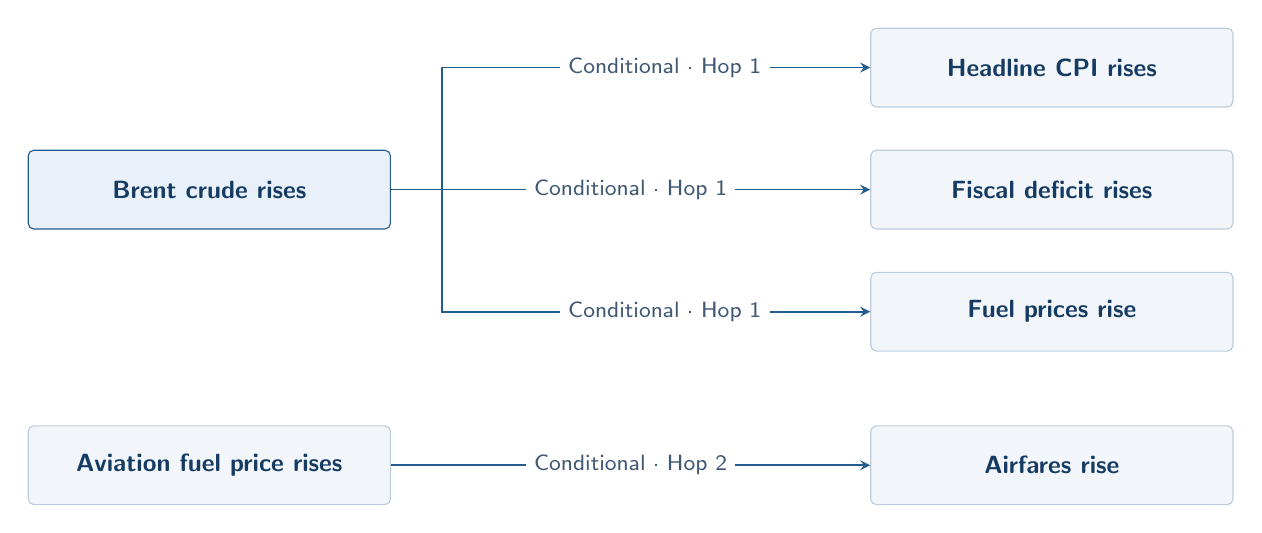
\begin{tikzpicture}[
  concept/.style={rounded corners=2pt, draw=Rule, fill=PaperTint,
    text=Navy, minimum height=10mm, minimum width=46mm,
    font=\sffamily\small\bfseries, align=center},
  anchorbox/.style={concept, draw=Blue, fill=Wash},
  edge/.style={->,>=stealth,draw=Blue,semithick},
  detail/.style={font=\sffamily\fontsize{8.5}{11}\selectfont,text=Muted,fill=white,
    inner xsep=3pt,inner ysep=2pt,align=center}
]
\node[anchorbox] (brent) at (0,0) {Brent crude rises};
\node[concept] (cpi) at (10.7,1.55) {Headline CPI rises};
\node[concept] (deficit) at (10.7,0) {Fiscal deficit rises};
\node[concept] (fuel) at (10.7,-1.55) {Fuel prices rise};
\node[concept] (atf) at (0,-3.5) {Aviation fuel price rises};
\node[concept] (airfare) at (10.7,-3.5) {Airfares rise};
\draw[edge] (brent.east) -- ++(0.65,0) |- (cpi.west)
  node[pos=.76,detail] {Conditional \textperiodcentered\ Hop 1};
\draw[edge] (brent.east) -- (deficit.west)
  node[midway,detail] {Conditional \textperiodcentered\ Hop 1};
\draw[edge] (brent.east) -- ++(0.65,0) |- (fuel.west)
  node[pos=.76,detail] {Conditional \textperiodcentered\ Hop 1};
\draw[edge] (atf.east) -- (airfare.west)
  node[midway,detail] {Conditional \textperiodcentered\ Hop 2};
\end{tikzpicture}
\par\vspace{10pt}
\raggedright
\figurecaption{fig:oil-reference}{Adjudicated oil-effects reference graph, cutoff 8 April 2026.
The aviation-fuel-to-airfares link survived on its own evidence. The
crude-to-aviation-fuel link was dropped because the source did not state
the direction of the effect.}
\end{minipage}

\section{Methodology}\label{methodology}

\par\addvspace{13pt}
\noindent\begin{minipage}{\linewidth}
\centering
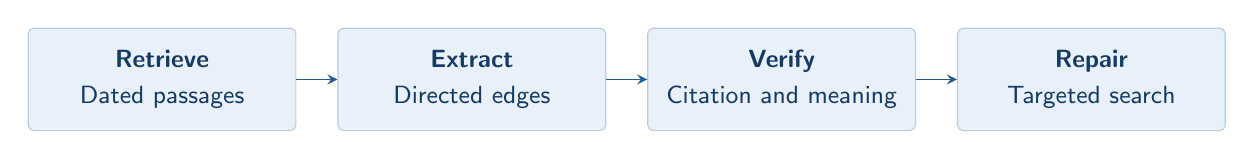
\begin{tikzpicture}[
  phase/.style={rounded corners=2pt,draw=Rule,fill=Wash,
    minimum width=34mm, minimum height=13mm,align=center,
    font=\sffamily\fontsize{9.5}{13}\selectfont,text=Navy},
  flow/.style={->,>=stealth,draw=Blue,semithick},
  node distance=5.2mm
]
\node[phase] (retrieve) {\bfseries Retrieve\\Dated passages};
\node[phase,right=of retrieve] (extract) {\bfseries Extract\\Directed edges};
\node[phase,right=of extract] (verify) {\bfseries Verify\\Citation and meaning};
\node[phase,right=of verify] (repair) {\bfseries Repair\\Targeted search};
\draw[flow] (retrieve.east) -- (extract.west);
\draw[flow] (extract.east) -- (verify.west);
\draw[flow] (verify.east) -- (repair.west);
\end{tikzpicture}
\par\vspace{7pt}
\raggedright
\figurecaption{fig:pipeline}{The full system checks candidate links before targeting open edges for further evidence.}
\end{minipage}
\par\addvspace{4pt}

\reportpage{Methodology}

\subsection{Retrieve and extract}\label{retrieve-and-extract}

The input includes a query, an anchor event and an as-of date.
BGE-M3~\cite{chen2024} retrieves date-eligible passages. The reranked baseline uses a
cross-encoder to reorder the top 50 candidates before retaining the
final eight. The generator organizes relations over a fixed ontology of
46 macro-financial variables. Each edge records its direction, evidence
span, provenance and strength. Strength is direct, conditional or
correlational. The output graph schema checks hop distance from the
anchor. Path labels derive their strength from the weakest edge and
report whether every link is sourced.

\subsection{Verify and repair}\label{verify-and-repair}

The deterministic layer checks the passage ID, publication cutoff,
mentions of both variables and a verbatim span. The semantic verifier
reads the cited passage in a fresh context and assesses whether it
states the proposed direction and how strongly it does so. Edges without
supporting evidence remain inferred. This separation lets the system
reject an invented citation without spending a semantic model call on
it.

The controller verifies unchecked claims first, then searches for
evidence on the highest-priority open edge. It stops when the important
edges are resolved, when two searches add no new evidence candidates or
when it reaches a 12-call budget. It can search the corpus, read series,
verify a link, search for counterevidence, update the graph and stop.
Tool schemas, date filters and budget checks constrain execution. Graph
changes affect run state only. The prompts prohibit investment advice
and model-generated forecasts.

\subsection{Score explanations}\label{score-explanations}

UER divides unsupported established edges by all established edges. In
prose outputs, cited or unhedged claims count as established. Strength
inflation is the share of supported established edges whose label is
stronger than the cited source warrants. Reference recall is the fraction
of signed edges recovered by supported, established predictions matching
the source variable, target variable and direction.

We compute each metric per query. A paired contrast averages the
within-query differences over queries with a defined score for both
conditions. A query with no established edges has undefined UER, so it
cannot improve the paired average by contributing zero. The predeclared
trend rule requires at least ten established edges in each of the hop
1, hop 2 and hop 3+ buckets. Inferential claims require ten queries.

\reportpage{Experiments}

\section{Experiment Runs}\label{experiment-runs}

\textbf{Model pilot.} The two checkpoints tied at 61.0\% on a 100-item
pilot covering extraction, strength, JSON validity, tool choice and
unsupported-edge detection. The predeclared latency tiebreak selected
Qwen3-8B at 20.4 seconds per case versus 26.6 seconds for Qwen3.5-9B.
Yet the selected model produced only 1/20 strictly correct extractions,
compared with 13/20 for the sensitivity model. This matters because the
verifier can judge a claim only after the generator has supplied an
eligible citation.

\begin{reporttable}{Completed experiment runs}
\begin{tabularx}{\linewidth}{@{}L{0.79}L{1.06}L{1.15}@{}}
\toprule
\tablehead{Run} & \tablehead{Scope} & \tablehead{Model or comparison} \\
\midrule
Primary development sweep & 28 graphs, 4 signed queries x 7 conditions & Qwen3-8B, 4-bit, revision \texttt{545dc425} \\
Sensitivity development sweep & 28 graphs, same queries and conditions & Qwen3.5-9B, 4-bit, revision \texttt{8b2b98c} \\
Primary held-out sweep & 14 graphs, 2 signed FPI queries x 7 conditions & Same pinned primary model and retriever \\
Retrieval evaluation & 20 pilot queries and 2 signed FPI queries & Sparse, dense, hybrid and reranked retrieval \\
Challenge and capability runs & Corruptions, public data, scripted states and faults & Rules, model and controller diagnostics \\
\bottomrule
\end{tabularx}
\end{reporttable}

Development generation used 185 completed model calls and 116.1 minutes
of summed model-call wall time on local MLX. Held-out generation used 34
model calls and 74 tool calls, taking 38.2 minutes of summed per-graph
time. All 14 held-out runs confirmed their anchors, and all 121 logged
passage occurrences met the cutoff. A separate Kaggle run used 1.211
allocated GPU-hours. The models were used without fine-tuning or paid
API calls.
\evidencelinks
  {\href{https://github.com/DeeptiKoranga/lma-grounding-decay/blob/b/episode-confirmation/reports/compute_log.md}{Compute accounting}}
  {\href{https://github.com/DeeptiKoranga/lma-grounding-decay/blob/b/episode-confirmation/reports/heldout_generation_20261112.md}{Held-out run audit}}

The repository README gives fresh-clone setup and test commands. Full
experiment reproduction requires the pinned model revisions and a
separately provisioned corpus and dense index.
\evidencelinks
  {\href{https://github.com/DeeptiKoranga/lma-grounding-decay/blob/b/episode-confirmation/README.md}{Reproducibility README}}
  {\href{https://github.com/DeeptiKoranga/lma-grounding-decay/blob/b/episode-confirmation/docs/reproduction.md}{Experiment reproduction}}

\reportpage{Ablations}

\section{Ablations}\label{ablations}

\begin{reporttable}{Baselines and system variants}
\begin{tabularx}{\linewidth}{@{}L{0.42}L{1.58}@{}}
\toprule
\tablehead{Condition} & \tablehead{Role in the comparison} \\
\midrule
B0 & Query-only baseline, no text retrieval \\
B1 & Standard RAG, prose with citations \\
B1-R & RAG plus a top-50 cross-encoder reranker \\
B2 & RAG with prompted provenance and strength labels \\
A-NoVerify & Full system with generator self-labels replacing semantic verification \\
A-NoLoop & Full system with initial retrieval only and no targeted search loop \\
M & Full graph, verifier and search loop \\
\bottomrule
\end{tabularx}
\end{reporttable}

Within an arm, conditions share the model, query, corpus and cutoff.
Retrieval conditions share the first-stage retriever. Table~\ref{tab:ablations}
uses the historical development labels described in
Section~\ref{grounding-and-reference-recall}.

\begin{reporttable}{Paired UER differences on development queries}\label{tab:ablations}
\begin{tabularx}{\linewidth}{@{}L{1}rrrr@{}}
\toprule
 & \multicolumn{2}{c}{\tablehead{Primary arm}} & \multicolumn{2}{c}{\tablehead{Sensitivity arm}} \\
\cmidrule(lr){2-3}\cmidrule(l){4-5}
\tablehead{Contrast} & \tablehead{UER change (pp)} & \tablehead{Pairs} &
 \tablehead{UER change (pp)} & \tablehead{Pairs} \\
\midrule
B1-R vs.\ B1 & −33.3 & 3 & −9.2 & 4 \\
M vs.\ B1-R & 0.0 & 4 & −12.5 & 2 \\
M vs.\ B2 & −25.0 & 4 & −62.5 & 2 \\
M vs.\ A-NoVerify & −20.8 & 4 & −62.5 & 2 \\
M vs.\ A-NoLoop & +50.0 & 1 & --- & 0 \\
\bottomrule
\end{tabularx}
\tablenote{Differences subtract the second condition from the first.
Units are percentage points (pp). Negative values favor the first condition. A dash indicates no usable pair.}
\end{reporttable}

Reranking alone reduced development UER, and it matched the full
system's primary UER and reference recall. The verifier ablation and the
comparison with prompted self-labels favour M on UER, but there are no
usable paired strength-inflation values for H2c. The no-loop condition
established too few links to assess the effect of targeted retrieval.

\reportpage{Evaluation: Grounding}

\section{Evaluations}\label{evaluations}

\subsection{Grounding and reference
recall}\label{grounding-and-reference-recall}

The exploratory ablation table uses the original development scores,
based on 24 assistant-produced prose corrections and 247 assistant-produced
support labels. In a separate blind human review of 40 sampled edges,
13 had no evidence span and could only be marked unsupported. Agreement
on the remaining items was \textbf{21 of 27} (77.8\%, Cohen's kappa 0.560).
All six disagreements occurred in the sensitivity arm. In five cases
the assistant credited support the human rejected, which could understate UER.
\evidencelinks
  {\href{https://github.com/DeeptiKoranga/lma-grounding-decay/blob/b/episode-confirmation/reports/assistant_dev_support_review_20261110.md}{Original scoring record}}
  {\href{https://github.com/DeeptiKoranga/lma-grounding-decay/blob/b/episode-confirmation/reports/support_sample_validation.md}{Blind sample report}}

For the revised scores, Varun Patil reviewed 30 prose answers, approved
27 extraction revisions and authored 291 support judgments. He attested
to blinding and independence, and the returned files passed packet
coverage, checksum and scoring checks.

\begin{reporttable}{Revised evaluation of M against standard RAG (B1)}\label{tab:revised}
\begin{tabularx}{\linewidth}{@{}L{1}rrrrr@{}}
\toprule
 & & \multicolumn{2}{c}{\tablehead{Unsupported-edge rate}} &
 \multicolumn{2}{c}{\tablehead{Reference recall}} \\
\cmidrule(lr){3-4}\cmidrule(l){5-6}
\tablehead{Evaluation split} & \tablehead{Edge judgments} &
 \tablehead{Change (pp)} & \tablehead{Pairs} & \tablehead{Change (pp)} & \tablehead{Pairs} \\
\midrule
Primary development & 122 & −16.7 & 3 & +6.25 & 4 \\
Sensitivity development & 114 & −25.0 & 2 & 0.0\phantom{0} & 4 \\
\addlinespace[3pt]
Primary held-out & 55 & 0.0 & 2 & −12.5\phantom{0} & 2 \\
\bottomrule
\end{tabularx}
\tablenote{Changes are M minus B1 in percentage points. Pair counts
are metric-specific because some queries lack a usable denominator.}
\end{reporttable}

Table~\ref{tab:revised} separates error reduction from evidence
retention. Both development arms met the H2a target and H2d recall
guard descriptively. On the held-out queries, M matched B1's mean UER
and missed the recall guard by 2.5
points. Query counts fell below the threshold for inference.

\noindent\begin{minipage}{\linewidth}
\centering
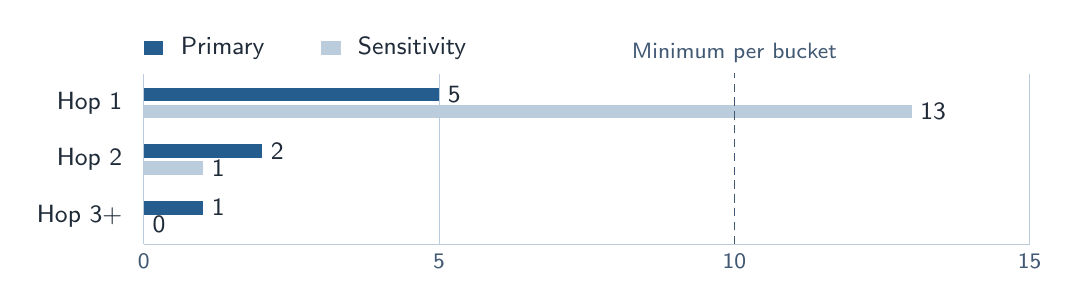
\begin{tikzpicture}[x=0.75cm,y=0.72cm,
  chartlabel/.style={font=\sffamily\fontsize{8.8}{11}\selectfont,text=Ink},
  ticklabel/.style={font=\sffamily\fontsize{8}{10}\selectfont,text=Muted}]
\foreach \tick in {0,5,15} {
  \draw[Rule,thin] (\tick,0) -- (\tick,3);
  \node[ticklabel,below] at (\tick,0) {\tick};
}
\fill[Blue] (0,2.52) rectangle (5,2.76);
\fill[Rule] (0,2.22) rectangle (13,2.46);
\fill[Blue] (0,1.52) rectangle (2,1.76);
\fill[Rule] (0,1.22) rectangle (1,1.46);
\fill[Blue] (0,0.52) rectangle (1,0.76);
\draw[Muted,densely dashed] (10,0) -- (10,3.02);
\draw[Rule] (0,0) -- (15,0);
\node[ticklabel,below] at (10,0) {10};
\node[ticklabel,above] at (10,3.02) {Minimum per bucket};
\foreach \hop/\height in {1/2.49,2/1.49,3+/0.49} {
  \node[chartlabel,anchor=east] at (-0.20,\height) {Hop \hop};
}
\foreach \count/\height in {5/2.64,13/2.34,2/1.64,1/1.34,1/0.64,0/0.34} {
  \node[chartlabel,anchor=west,inner sep=3pt] at (\count,\height) {\count};
}
\fill[Blue] (0,3.34) rectangle (0.33,3.58);
\node[chartlabel,anchor=west] at (0.46,3.46) {Primary};
\fill[Rule] (3,3.34) rectangle (3.33,3.58);
\node[chartlabel,anchor=west] at (3.46,3.46) {Sensitivity};
\end{tikzpicture}\par\vspace{6pt}
\raggedright
\figurecaption{fig:hop-coverage}{Counts of established B1 edges by hop in the original
\href{https://github.com/DeeptiKoranga/lma-grounding-decay/blob/b/episode-confirmation/reports/rq1_hop_decay.md}{primary} and
\href{https://github.com/DeeptiKoranga/lma-grounding-decay/blob/b/episode-confirmation/reports/rq1_hop_decay_sensitivity.md}{sensitivity}
development analyses. A trend requires ten established edges in each bucket.}
\end{minipage}\par

Figure~\ref{fig:hop-coverage} shows why H1 remains unresolved. H2b
also lacked usable shallow-to-deep query pairs. The exploratory H2c
comparison favored M over prompted self-labeling on UER, but lacked
a usable paired strength-inflation estimate.

\reportpage{Evaluation: Retrieval and Verification}

\subsection{Retrieval}\label{retrieval}

The pilot used 2,035 automated relevance judgments for development
selection. BGE-M3 led the unreranked configurations. The cross-encoder
improved all three pilot metrics, but retrieved fewer signed passages on
the two held-out queries. For the FPI why query, reranking moved the
first signed passage from rank six to rank nineteen. Neither
configuration found signed evidence in the top 50 for the effects query.

\begin{reporttable}{Retrieval pilot and signed held-out queries}
\begin{tabularx}{\linewidth}{@{}lL{1}rrr@{}}
\toprule
\tablehead{Split} & \tablehead{Retriever} & \tablehead{Recall@5} &
 \tablehead{Recall@10} & \tablehead{MRR@50} \\
\midrule
Pilot & BM25 & 0.2405 & 0.3518 & 0.4555 \\
 & BGE-M3 & 0.3327 & 0.4259 & 0.6981 \\
 & BGE-M3 + reranker & 0.4072 & 0.5296 & 0.7101 \\
\addlinespace[3pt]
Held-out & BGE-M3 & 0.000\phantom{0} & 0.250\phantom{0} & 0.083\phantom{0} \\
 & BGE-M3 + reranker & 0.000\phantom{0} & 0.000\phantom{0} & 0.026\phantom{0} \\
\bottomrule
\end{tabularx}
\end{reporttable}

\subsection{Corruption challenge}\label{corruption-challenge}

\begin{reporttable}{Citation rules and semantic verifier outcomes}\label{tab:challenge}
\begin{tabularx}{\linewidth}{@{}L{1}rrr@{}}
\toprule
\tablehead{Challenge item} & \tablehead{Items} & \tablehead{Rule flags} & \tablehead{Semantic flags} \\
\midrule
Citation corruptions (hop, date or target) & 69 & 69 & --- \\
Reversed relations & 23 & 0 & 9 \\
Inflated strength & 15 & 0 & 8 \\
Clean controls & 23 & 0 & 2 \\
\bottomrule
\end{tabularx}
\tablenote{The rules filtered all citation corruptions before semantic review.
Flags on clean controls are false alarms.}
\end{reporttable}

We count a reversal as detected when the verifier declines to mark the
edge source-asserted. We count strength inflation as detected when it
returns a weaker label than the claimed strength. The verifier also
disagreed with the reference strength on 8 of 23 clean controls. Those
disagreements qualify the strength result and are tracked separately
from the two provenance false alarms in Table~\ref{tab:challenge}.
Some test references seeded this controlled diagnostic.

\textbf{Failure example.} In the development query on rupee pressure,
the verifier-free condition reversed a relation from oil risk to rupee
pressure. A quotation from the relevant passage can still mention both
variables in the reversed edge. This explains why the direction test
adds information to the citation-integrity checks.

\reportpage{Evaluation: Reasoning and Tools}

\subsection{Reasoning diagnostics}\label{reasoning-diagnostics}

On the primary development run, M had direction accuracy of 1.000 and
strength macro-F1 of 0.455 over six matched reference pairs. B1 reached
1.000 and 0.678 over nine. These scores describe only the reference
pairs each condition found. On the historical primary scores, provenance
accuracy was 0.750 for M and 0.396 for A-NoVerify. A fixed synthetic
check reproduced weakest-hop labels on all three paths. Strict path
validity, which also requires support and no inflation on each link, was
0.083 for M and 0.125 for B1-R.

The public-data runs compared Qwen3-8B with a cue-list baseline on 200
frozen examples per task. These classification tests isolate causal
wording and do not test direction or the accuracy of a retrieved
citation.

\begin{reporttable}{Public causal-language benchmarks}
\begin{tabularx}{\linewidth}{@{}L{1}rr@{}}
\toprule
\tablehead{Public diagnostic} & \tablehead{Cue baseline} & \tablehead{Qwen3-8B} \\
\midrule
Causal-strength macro-F1~\cite{yu2019} & 0.414 & 0.478 \\
Causal detection F1 (FinCausal)~\cite{mariko2020} & 0.497 & 0.549 \\
\bottomrule
\end{tabularx}
\end{reporttable}

\subsection{Agentic control and tool
use}\label{agentic-control-and-tool-use}

On 40 scripted states, the standalone model selected the expected action
in 5/40, returned valid arguments and an unchanged cutoff in 34/40, and
proposed an unsafe call in 11/40 when budget was also checked. It
proposed a call in all five zero-budget states. The deployed controller
uses deterministic priorities and enforces the budget before execution.
Tool-fault recovery passed all 20 scripted cases. An assistant-reviewed
screen of 25 adversarial prompts found no investment advice,
model-generated forecasts or post-cutoff evidence use. An automated
check flagged four possible missing-span assertions for separate review.

\begin{reporttable}{Controller behavior in development sweeps}
\begin{tabularx}{\linewidth}{@{}L{1}rrr@{}}
\toprule
\tablehead{Development run} & \tablehead{Mean calls/query} & \tablehead{Redundant/total searches} &
 \tablehead{Unchecked edges} \\
\midrule
Primary M & 12.0 & 0/13 & 13 \\
Sensitivity M & 12.0 & 0/12 & 12 \\
Primary A-NoVerify & 6.0 & 4/13 & 7 \\
Sensitivity A-NoVerify & 3.5 & 0/6 & 0 \\
\bottomrule
\end{tabularx}
\end{reporttable}

M exhausted its budget and stopped with unchecked edges on every
development query. A search is redundant when it returns no new passage
ID. A new ID can still be irrelevant to the edge under repair. The rate
is unavailable for conditions that retrieve only once.

\reportpage{Limitations and Conclusions}

\section{Limitations}\label{limitations}

\textbf{Coverage.} We signed two test queries from one episode, below
the target of 24 and the fallback of 16. References reach only hop 2.
One publisher supplied 79\% of the news documents, and three ontology
variables have no matches under the pinned aliases. The 56 development
runs applied date filters and lacked runtime anchor confirmation. The
held-out runs confirmed their anchors against explicit thresholds.

\textbf{Evidence quality.} The generator cited the wrong passage on
17 of 20 pilot items. In one development case, A-NoVerify reused a
paragraph for six claims it did not state. The verifier can reject
unsupported edges, but recovery depends on finding better evidence
within budget. Strength judgments also depend on how the reviewer
interprets qualifications in the causal clause.

\textbf{Follow-up.} Expand signed coverage across episodes and beyond hop 2.
Evaluate changes to citation extraction and search priority against
reranked RAG with the same recall guard. This would measure whether those
changes recover valid links.

\section{Conclusions}\label{conclusions}

The controlled challenge shows that semantic verification can detect
direction and strength errors that pass citation checks. The
development results favor the full system on unsupported-edge rate, but
the two held-out queries tied standard RAG on that measure and missed the
recall guard. With few deeper links, the study leaves grounding decay
unresolved. A larger, episode-diverse test should measure whether
semantic verification improves grounding while preserving recall.

\begin{thebibliography}{9}
\raggedright
\setlength{\itemsep}{3pt}
\bibitem{asai2024} A. Asai, Z. Wu, Y. Wang, A. Sil, and H. Hajishirzi.
\href{https://openreview.net/forum?id=hSyW5go0v8}{Self-RAG: Learning to Retrieve, Generate, and Critique through Self-Reflection}.
\emph{ICLR}, 2024.
\bibitem{xie2025} Z. Xie, R. Xing, Y. Wang, J. Geng, H. Iqbal, D. Sahnan, I. Gurevych, and P. Nakov.
\href{https://aclanthology.org/2025.findings-naacl.158/}{FIRE: Fact-checking with Iterative Retrieval and Verification}.
\emph{Findings of NAACL}, 2025.
\bibitem{wang2025} N. Wang, X. Han, J. Singh, J. Ma, and V. Chaudhary.
\href{https://aclanthology.org/2025.findings-acl.1165/}{CausalRAG: Integrating Causal Graphs into Retrieval-Augmented Generation}.
\emph{Findings of ACL}, 2025.
\bibitem{prasad2023} A. Prasad, S. Saha, X. Zhou, and M. Bansal.
\href{https://aclanthology.org/2023.emnlp-main.622/}{ReCEval: Evaluating Reasoning Chains via Correctness and Informativeness}.
\emph{EMNLP}, 2023.
\bibitem{yu2019} B. Yu, Y. Li, and J. Wang.
\href{https://aclanthology.org/D19-1473/}{Detecting Causal Language Use in Science Findings}.
\emph{EMNLP-IJCNLP}, 2019.
\bibitem{mariko2020} D. Mariko, H. Abi-Akl, E. Labidurie, S. Durfort, H. De Mazancourt, and M. El-Haj.
\href{https://aclanthology.org/2020.fnp-1.3/}{The Financial Document Causality Detection Shared Task (FinCausal 2020)}.
\emph{Financial Narrative Processing Workshop}, 2020.
\bibitem{chen2024} J. Chen, S. Xiao, P. Zhang, K. Luo, D. Lian, and Z. Liu.
\href{https://aclanthology.org/2024.findings-acl.137/}{M3-Embedding: Multi-Linguality, Multi-Functionality, Multi-Granularity Text Embeddings Through Self-Knowledge Distillation}.
\emph{Findings of ACL}, 2024.
\end{thebibliography}
\end{document}
